\documentclass{article}

\usepackage[margin=2.5cm,left=2cm,includefoot]{geometry}
\usepackage{graphicx}
\usepackage{float}
\usepackage[space]{grffile}
\usepackage{hyperref}
\usepackage[export]{adjustbox}
\usepackage{multicol}
\usepackage{caption}
\usepackage{hyperref}
\usepackage{listings}
\usepackage{vhistory}
\usepackage{titlesec}

\setcounter{secnumdepth}{4}

\titleformat{\paragraph}
{\normalfont\normalsize\bfseries}{\theparagraph}{1em}{}
\titlespacing*{\paragraph}
{0pt}{3.25ex plus 1ex minus .2ex}{1.5ex plus .2ex}

% Header and footer
\usepackage{fancyhdr}
\pagestyle{fancy}

\rhead{COS301}
\lhead{Architecture Requirements}
\fancyfoot[R]{Page \thepage}

\renewcommand{\headrulewidth}{2pt}
\renewcommand{\footrulewidth}{1pt}

\begin{document}

	\begin{titlepage}
		\begin{center}
			
\includegraphics[width=10cm]{images/marketlead_3.png}  \\
			[0.5cm]
			\huge{
			Architectural Requirements, Architecture Design and Non-Functional Requirements\\
			}

			\line(1,0){300}\\
			[0.2cm]
			\LARGE{Project: Insurance profiling from social media\\
			Client: RetroRabbit} \\
			\line(1,0){300}\\
			\LARGE{Team: Valknut Solutions}\\
			[1.0cm]
			\large
			{
			\begin{itemize}
				\item 13054903 - Charl Jansen van Vuuren
				\item 13044924 - Kevin Heritage
				\item 13176545 - Quinton Weenink\\
			\end{itemize}
			}
			\textsc{\large}\\
		[2.0cm]
		\textsc{\large  Department of Computer Science}\\
		[0.5cm]
		\textsc{\large \today}\\
		\end{center}

		%\begin{figure}[H]}
		%\centering
		%\includegraphics[{imagename}
		%\end{figure}\

	\end{titlepage}
	\cleardoublepage
	\tableofcontents
	\cleardoublepage

		% Start of the revision history table
	\begin{versionhistory}
  		\vhEntry{1.0}{27.05.2016}{CJvV,KH,QW}{Created}
  		\vhEntry{1.1}{27.07.2016}{CJvV,KH,QW}{Grammar errors, Introduction, Scope, Vision, Access channel, Quality requirements, Integration Requirements (API, Protocols, API Quality requirements), Architectural tactics(Security) and Architectural pattern changes}
  		\vhEntry{1.2}{07.09.2016}{CJvV,KH,QW}{Updated introduction, scope, Access channel requirements, Integration quality requirements, architectural Tactics, Architectural pattern}
  		\vhEntry{1.3}{05.10.2016}{CJvV,KH,QW}{Updated front-page with logo, updated introduction, vision, scope,Access channel requirements}
	\end{versionhistory}

\pagebreak

\section{Introduction}
 Insurance profiling and risk analysis often require large amounts of data to generate in-depth profiles, our project aims to eliminate the need for vast amounts of data gathering by utilising a user's social media information, based on advertisement forms and the integration of a Facebook and Wechat messenger bot.\\ This includes the managing and processing of these leads from the marketing and analysis viewpoints.

\section{Scope of system}
The project as it is currently specified is an application that will allow insurance companies the ability to get data from lead data provided via lead advertisements on Facebook.
A user fills in a Facebook advertisement to purchase short term insurance based on Facebook's advertisement audience algorithm. \\
Further access points are available by means of a personalized Facebook messenger bot and Wechat messenger integration.\\ The use of messenger bots allow for a more personalized look and feel, as the user can supply information by means of talking to the bot. \\ \\
This data will be used to charge the users for the insurance that they have signed up for while also providing the application with some basic data that can later be used to analyse the users and the data they provided. \\
An analyst would be able to log into our system and generate risk statistics for a certain advertisement based on certain criteria, this information gives the insurance company the ability to charge and adapt their sale and costs based on popular advertisements.\\ \\
This information will be available based on API calls to the database or through a Web front-end for analysts.\\
A live dashboard for marketing follow ups will allow marketers the ability to see unprocessed leads and live graphs.


\section{Vision}
We seek to implement a real time marketing and lead gathering application with multiple integration points with social media and other formats. 
A business can manage and respond to leads and analyze their current customers and audience. 
We expose and link companies to their future customers in an easy and pluggable manner.

\pagebreak

\section{Architectural Requirements}
	\subsection{Access channel requirements}
\subsubsection{User:}
	\begin{enumerate}
		\item A user will fill in an advertisement form on Facebook, or chat with a messenger bot to supply the information specified and submit this data.
		\item This data can also be filled in via the website form.
		\item The necessary data will be gathered and saved in the database.
		\item The system will analyze the data and send the user a response via email if they qualified for the insurance.
		\item A sales person will contact the specified user with further instructions.
	\end{enumerate}
\subsubsection{Analyst:}
	\begin{enumerate}
		\item An analyst would log into the system with a required username and password authorization
		\item Selection criteria to generate a report will be presented to the analyst.
		\item The analyst will be able to filter the report/graph/statistics based on certain specified criteria.
		\item Options for exporting the data will be available in different formats.
	\end{enumerate}
\subsubsection{Marketer:}
	\begin{enumerate}
		\item A marketer will supply the necessary  authorization to access the dashboard.
		\item A number of live graphs will be presented to the marketer to see new leads and user signups.
		\item The marketer will be able to see a list of unprocessed leads to follow up on
	\end{enumerate}	

\subsubsection{Further access channel specification include:}
	\begin{itemize}
		\item The website will be accessible from, and optimized for all web-browsers including mobile phone browsers.
		\item The possibility of developing a mobile application will be considered as per the client's request.
		\item The website will be accessible via the majority of operating systems if such an operating system has access to a supported web-browser.
		\item Facebook advertisement integration will be accessible via the normal Facebook access channels.
		\item Facebook messenger integration will be accessible via the Messenger application.
		\item Wechat integration will be available via the Wechat messenger platform.
	\end{itemize}


	\subsection{Quality Requirements}
		\paragraph{The tactics used to address these quality requirement issues are discussed in Section \ref{subsec:tactics}}
		\subsubsection{Performance}
		\begin{itemize}
			\item A user should be able to request a quote in less than 5 minutes. This is easily achieved by means of the Facebook advertisement and will only be user-network dependent.
			\item Once the REST API call is made, it saves the user's data in our database, increasing the efficiency of future requests and processing of the data.
			\item The need to do external API calls will be minimized, increasing performance.
			\item Tactics: Section \ref{subsec:performancetactic}
		\end{itemize}
		\subsubsection{Security}\label{subsubsec:security}
		\begin{itemize}
			\item Security is our most important architectural requirement. A user's personal information is used to generate these risk profiles and as a result the user will trust that this information is not shared with other parties, and properly secured.
			\item Only authorised persons will have access to generated statistics and access to the database and API will be restricted to authorized analysts and administrators only.
			\item The Heroku server's adds an extra layer of security with regards to random generation of usernames and passwords for access to the database.
			\item Tactics : Section \ref{subsec:security}
		\end{itemize}
		\subsubsection{Scalability}
		\begin{itemize}
			\item Since this project is a web-based solution, the possibility of multiple concurrent users should be considered.
			\item The server should account for a vast amount of concurrent users.
			\item As per integratability \ref{subsubsec:integratability}, the ability to change the risk analysis algorithm as needed should be considered for a future scalable solution.
			\item Tactics : Section \ref{subsec:scalability}
		\end{itemize}

		\subsubsection{Integratability}\label{subsubsec:integratability}
		\begin{itemize}
			\item The project will integrate with Facebook and utilise it as the primary data provider.
			\item The ability to integrate with other social media platforms should be considered and modularised accordingly, to ensure seamless future integration.
			\item The ability to change the risk analysis algorithm as needed should be considered.
			\item Integration includes the connection from the website to the profiling engine and back to the website as a report.
			\item Integration with Facebook's advertisements API forms a major part of this release.
			\item Tactics : Section \ref{subsec:accesib}
		\end{itemize}

		\subsubsection{Reliability}
		\begin{itemize}
			\item Since our solution is mainly web-based, the platform as a service (PaaS) offered by Heroku will ensure the website is always up to date and reliable.
			\item Tactics : Section \ref{subsec:reliability}
		\end{itemize}

		\subsubsection{Maintainability}
			The system will make use of a database with massive amounts of data.\\ To ensure optimal performance, this data will need to be maintained and normalised on a regular basis.

		\subsubsection{Auditability}
		\begin{itemize}
			\item All actions performed in the system should be traceable to the user that performed them.
			\item The user's IP  will be logged as to have a form of accountability in the persistence of the data.
		\end{itemize}

		\subsubsection{Cost}
		The majority of our platform is open-source, except for:
		\begin{itemize}
			\item Heroku hosting if the commercial version is used
			\item Travis CI if the commercial version is used
			\item Facebook's advertisement campaigns are billed monthly if the advertisement is to be live.
		\end{itemize}
		The current free versions of these platforms are used. \\
		The Facebook advertisements are currently not live as this project is still in the development stage.

		\subsubsection{Usability}
		\begin{itemize}
			\item The platform is being developed with efficiency in mind, as a result the input and response of the website should be visually pleasing and simple to use.
			\item Further integration with the Facebook ad system will increase usability, as the user will be able to generate a report from their Facebook dashboard, without the need to log in to our website.
			\item The Facebook messenger integration allows a more fulfilling user experience as it eliminates the normal form structure of capturing data.
		\end{itemize}

		\subsubsection{Flexibility}
		\begin{itemize}
			\item The system must be usable on any internet browser (including mobile phone browsers).
			\item The system must include the ability to change the risk analysis algorithm. Insurance profilers can use this to their advantage to generate more thorough risk profiles.
			\item Tactics : Section \ref{subsec:modifi}
		\end{itemize}

		\subsubsection{Compatibility}
		\begin{itemize}
			\item The use of Travis CI tests ensures the latest features are compatible with the specified versions of NodeJS.
			\item Unit tests constantly test the system's compatibility as part of the continuous integration model.
		\end{itemize}
		


	\subsection{Integration requirements}
		\subsubsection{API specifications}
		\begin{itemize}
		
		
			\item The Facebook advertisement and marketing API form a major part of this project.
			
			\item The Facebook Pages API forms part of this.
			\item The use of Facebook's Graph API by means of the Node package.
			\item An alternative is to use Curl based calls to interact with these APIs.
			\item The method of interacting with the API will be to parse the JSON string that will be returned by the Facebook server.
			\item It is also possible to get the access token using this method (a string of characters giving you access to a persons  account with the permissions specified).
			\item Facebook messenger bot integration is supplied by means of the Facebook messenger api \href{https://developers.facebook.com/docs/messenger-platform}{Facebook Messenger}
			\item Wechat integration is supplie by means of the Official account developer platform API, for Wechat. \href{http://dev.wechat.com/}{Wechat API}
		\end{itemize}
			Regarding the use of  access tokens, a Facebook page Access token and Facebook user access token will be used. These Access Token should also have the longest lifetime possible to be able to update user data for as long as possible.

			\href{https://developers..com/docs/-login/access-tokens}{Access Tokens}
			\begin{itemize}
				\item The access tokens generated via web logins are short-lived, but one can convert them to long-lived tokens.
				\item Apps with Standard access to Facebook's Marketing API when using long-lived tokens will receive long-lived tokens that don't have an expiry time.
				\item For security to validate some data we may need to gain Application access tokens. These tokens are only for the developers of the application not for general public.
				\item To generate an app access token:
					\begin{verbatim}
						/oauth/access_token?
					     client_id={app-id}
					    &amp;client_secret={app-secret}
					    &amp;grant_type=client_credentials
					\end{verbatim}
				\item Once again the app secret should be kept safe and hidden from users
			\end{itemize}

			
	\pagebreak
		\subsubsection{Protocols}
		The system will include the use of these protocols:
		\begin{itemize}
			\item HTTP/HTTPS - (Secure) Hypertext Transfer Protocol
			\item TCP/IP - Transmission Control Protocol/Internet Protocol
			\item FTP(Possibly) - File Transfer Protocol
			\item SSL - Secure Socket Layer
			\item SMTP - Simple Mail Transfer Protocol(with  SSL)
		\end{itemize}
		The request for comment pages of these protocols can be accessed via:
		\begin{itemize}
			\item\href{https://tools.ietf.org/html/rfc2616}{HTTP}
			\item\href{https://tools.ietf.org/html/rfc2660}{HTTPS}
			\item\href{https://www.ietf.org/rfc/rfc793.txt}{TCP}
			\item\href{http://www.ietf.org/rfc/rfc0791.txt}{IP}
			\item\href{https://www.ietf.org/rfc/rfc959.txt}{FTP}
			\item\href{https://tools.ietf.org/html/rfc6101}{SSL}
			\item\href{https://tools.ietf.org/html/rfc821}{SMTP}
		\end{itemize}


		\subsubsection{Integration Quality Requirements}
		\paragraph{The below mentioned use of the word Facebook is related to the Facebook advertisement integration and the messenger platform}
		As mentioned in \ref{subsubsec:integratability}, integration with Facebook will be a major feature, as such this integration is subject to quality requirements in the form of:
		\begin{itemize}
			\item Reliability - The Facebook API, Wechat API and Messenger API server must be available at all times as this forms a major part of the system.
			\item Auditability - The use of the Facebook developer application ID allows for auditability as to the use of the Facebook API in our system. The developer application ID allows Facebook to obtain information on the current use of their API with regards to our system. Wechat uses their own form of auditability similar to the Facebook method.
			\item Performance - Our system's performance in certain areas, is limited to the use of the above mentioned APIs. The API systesm must respond before our system can analyse the data.
			\item Security - Facebook's API has security measures in place to ensure that the Advertisement's data isn't accessed without authorization. This consent is granted by means of a permission request to the Analyst's Facebook page before we can obtain any information. The safeguard of this information is a major concern as mentioned in \ref{subsubsec:security}.
			\item Maintainability - The system must be maintained on a bi-yearly basis as to ensure the latest version of the API is used and no deprecated functions are used. The use of deprecated functions can cause problems in future use of the system.
		\end{itemize}


	\subsection{Architecture Constraints}
	Our client limited our technologies to:
	\begin{itemize}
		\item An ASP.net web solution with a Microsoft SQL Server database system.
		\item A NodeJS web solution with a PostgreSQL database system.
		\item The use of a platform as a services (PaaS) hosting solution, Heroku.
		\item We have the freedom to use the Facebook SDK in any language except for PHP as mentioned below.
	\end{itemize}
	Our client specifically constrained the use of:
		\begin{itemize}
		\item PHP code in any way.
		\item MySQL, NoSQL database systems.
		\end{itemize}
	Other constraints in terms of architecture include:
	\begin{itemize}
		\item Browser independence, to ensure any web-client can make use thereof.
		\item Operating system independence.
		\item The system should be as time efficient as possible
		\end{itemize}
\pagebreak

	\section{Initial Architecture Design}

	The below mentioned architecture specifies an initial architecture design from a high-leve l standpoint, of the system as it is currently understood at this stage in development and design. Any and all architectural components, tactics and responsibilities listed are subject to change and are at a level which attempts to provide the best description of what is currently intended to be the insurance profiling system.

	\subsection{Architectural tactics}\label{subsec:tactics}

	Due to the fact that the underlying architecture has of yet not been clearly specified, the investigation into the best suited tactics for this architecture can not be concretely concluded. The following is by no means a representation of the implemented tactics but it is currently what best helps the system achieve its quality requirements. The below listed tactics are currently the main tactics we aim to implement or the responsibility of the dependencies we aim to utilize.

		\subsubsection{Modifiability and Flexibility}\label{subsec:modifi}
		What is certain, is that the above mentioned quality requirements will need to be addressed in a manner which allows for a system that is both highly modular and configurable, in order to allow the analysts of the data set to properly assess and tweak the tools that we aim to provide to them.

		\begin{itemize}
			\item Flexibility support: automated builds, automated testing and automated environment configuration
			\item Service provider flexibility: dependency injection
			\item Process flexibility: pipes and filters, responsibility localization
		\end{itemize}
		\subsubsection{Performance}\label{subsec:performancetactic}
		\begin{itemize}
		\item Object Relational mapping for database calls increase performance
		\item NodeJS makes use of Asynchronous callbacks to increase performance and not slow down other calls 
		\end{itemize}
		\subsubsection{Accessibility and Integratability}\label{subsec:accesib}
		\begin{itemize}
			\item Providing access: providing proxies, supporting standard communication protocols (REST calls)
		\end{itemize}

		\subsubsection{Security}\label{subsec:security}
		\begin{itemize}
			\item Resisting attacks: authentication, authorization, minimizing access channels, minimize complexity and enforcing secure defaults
			\item Detecting attacks: auditing, logging and integrity checking
			\item Recovering: restore states, dropping
			\item Hashing of passwords
			\item Adding secret token to access tokens
		\end{itemize}

		\subsubsection{Reliability}\label{subsec:reliability}
		\begin{itemize}
			\item Preventing faults: resource locking, testing framework, contracts based
			\item Detect faults: logging, deadlock detection and error/exception communication
			\item Recovery: rollback, backups and passive redundancy
			\item Version based branching to enable rollback functionality
		\end{itemize}

		\subsubsection{Scalability}\label{subsec:scalability}
		\begin{itemize}
			\item Resource demand: indexing, paging, query optimization
		\end{itemize}

	\subsection{Architectural components addressing architectural responsibilities}
		\begin{itemize}
		%\item that of providing an environment for specifying and executing reports to a reporting frame-work,
		\item Providing human access channels and external systems web access to the system services which in turn grants access to a web services framework such as a custom REST api,
		\item Providing users access through a browser to a web application framework. Node.js has such a framework called express.js and AngularJS.
		\item In order to provide hosting for business logic processes, an application server will be hosted by Heroku.
		\item Persistence of objects will be stored in an object-relational database management system called PostgreSQL.
		\item The responsibility of providing the persistence provider access to the persistence API by means of the Sequelize ORM.
		\end{itemize}

\pagebreak
	\subsection{Infrastructure}
	\subsubsection{Architectural (structural) patterns}
	\begin{itemize}
	
	
	\item In order to promote flexibility as well as testability, a hybrid pattern will be used, with key-traits from the  layered architectural pattern and the Model-View-Controller pattern.
	\item The layered approach allows for future development to change tactics (business logic tactics) and allows for the decoupling of different functions. 
	\item The Model-View-Controller pattern allows for a understandable and testable system, with proper modularization.
	MVC includes the ability to generate new views for the web based front-end efficiently. See Figure \ref{fig:techstack}
	\item Decoupling is crucial in order for the system to remain within its architectural concern boundaries, which will rely heavily on a modular configurable system.  
	\end{itemize}
	\subsubsection{Concepts and constraints for application components}
	Application components will not be deployed at the first level of granularity. Any application components will be hosted within the architectural components.
	\begin{figure}[H]
		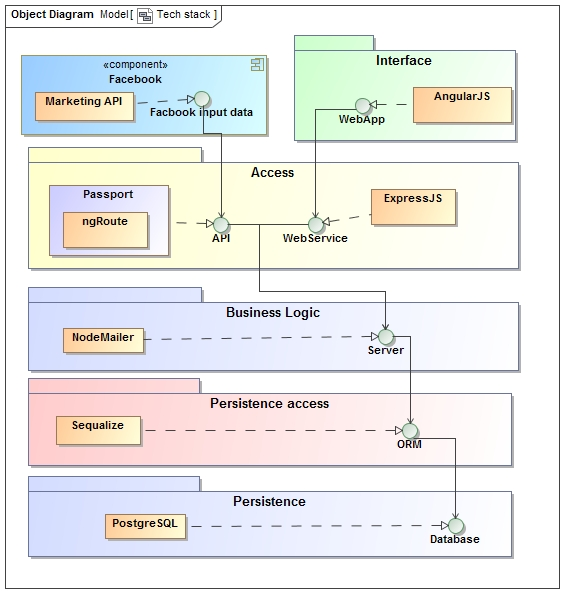
\includegraphics[width=\textwidth]{images/obj__Tech_stack.jpg}  \\
		\caption{Hybrid architectural pattern : Insurance Profiling}
		\label{fig:techstack}
	\end{figure}






\end{document}
